\documentclass{beamer}
\usepackage[utf8]{inputenc}
\usepackage{amsmath, pdfpages, pdflscape, lscape, color, listings, hyperref, amssymb, graphicx,textcomp,varioref, afterpage, subcaption, float, bm, tikz, multicol} 

\global
\newcommand{\Fig}[1]{Figure \ref{#1}}
\newcommand{\fig}[1]{figure \ref{#1}}
\newcommand{\tab}[1]{table \ref{#1}}
\newcommand{\eq}[1]{equation \ref{#1}}
\newcommand{\Eq}[1]{Equation \ref{#1}}
\newcommand{\alg}[1]{algorithm \ref{#1}}
\newcommand{\Alg}[1]{Algorithm \ref{#1}}
\newcommand{\chp}[1]{chapter  \ref{#1}}
\newcommand{\Chp}[1]{Chapter  \ref{#1}}
\newcommand{\e}[1]{\cdot 10^{#1}}
\newcommand{\h}{\hbar}
\newcommand{\der}[2]{\frac{\partial #1}{\partial #2}}
\newcommand{\dder}[2]{\frac{\partial^2 #1}{\partial #2^2}}
\newcommand{\p}{\boldsymbol{P}}
\newcommand{\q}{\boldsymbol{q}}

\newcommand{\norm}[1]{\left\lVert#1\right\rVert_{\!Q}}
\newcommand{\inner}[1]{\left\langle#1\right\rangle_{\!Q}}
\newcommand{\coef}[2]{\frac{\inner{#1,#2}}{\norm{#2}^2}}

\DeclareMathOperator*{\argmin}{argmin}
\DeclareMathOperator*{\argmax}{argmax}

\newcommand{\E}[1]{\mbox{E}\!\left(#1\right)}
\newcommand{\Var}[1]{\mbox{Var}\!\left(#1\right)}
\newcommand{\Cov}[1]{\mbox{Cov}\!\left(#1\right)}


\newenvironment{test}[1]
{
 \usebackgroundtemplate{}
 \color{gray!30!black}
   \begin{tikzpicture}[remember picture, overlay]
     \node[anchor = center, opacity=.25] (image) at (current page.center) {
\includegraphics[scale=0.25]{chaospy_logo.jpg}};
   \end{tikzpicture}
 \begin{frame}[fragile,enviroment=chaospy]
   
}
{
 \end{frame}
}

\lstset{
escapeinside=||
}


\newenvironment{chaospy}[1]
{\color{gray!30!black}
     \color{gray!30!black}
     \usebackgroundtemplate{
   \begin{tikzpicture}[remember picture, overlay]
     \node[anchor = center, opacity=.25] (image) at (current page.center) {
\includegraphics[scale=0.25]{chaospy_logo.jpg}};
   \end{tikzpicture}}
     \begin{frame}[fragile,environment=chaospy]
    \frametitle{{#1}}}
{\end{frame}}


\definecolor{keywords}{RGB}{255,0,90}
\definecolor{comments}{RGB}{0,0,113}
\definecolor{red}{RGB}{160,0,0}
\definecolor{green}{RGB}{0,150,0}
 
\usetheme{kalkulo}

\graphicspath{{./figures/}}


\title{Polynomial chaos expansions part 2: Practical Implementation}
\author{Jonathan Feinberg and Simen Tennøe}


\begin{document}



\begin{frame}
  \maketitle
\end{frame}

\begin{frame}
 \frametitle{Repetition of our naive problem}
  We have a simple differential equation
  \begin{align*}
    \frac{d u(x)}{dx} & =-au(x),\qquad u(0) = I,
  \end{align*}
  \pause
  With the solution:
  \[u(x) = Ie^{-ax}\]
  \pause
  where
   \[a \sim \text{Uniform(0, 0.1)}, \qquad I \sim \text{Uniform(8, 10)}\] 
\end{frame}


\begin{chaospy}{Repetion of teaser from last lecture}
    \scriptsize
    % TODO
    % high: make it 2-D problem
 \begin{lstlisting}[language=python]
 def u(x,a, I):
  return I*np.exp(-a*x)
|\pause| 
a = cp.Uniform(0, 0.1)
I = cp.Uniform(8, 10)
dist = cp.J(a,I)|\pause|
|\pause| 
P = cp.orth_ttr(2, dist)
|\pause|
nodes, weights = \
    cp.generate_quadrature(3, dist, rule="G")

x = np.linspace(0, 10, 100)
solves = [u(x, *node) for node in nodes.T]

u_hat = cp.fit_quadrature(P, nodes, weights, solves)

mean, var = cp.E(u_hat, dist), cp.Var(u_hat, dist)
\end{lstlisting}
\end{chaospy}


\begin{frame}
    \frametitle{Polynomial chaos expansions have a very fast
    convergence rate}
 % TODO
 % high: include error formula
 % med: legend lower right
 % med: figsize
%  \begin{center}
%   $   \varepsilon_E = \int_0^{10}|E(u) - E(\hat{u})|\,dx \qquad
%    \varepsilon_{Var} = \int_0^{10}|Var(u) - Var(\hat{u})|\,dx$
%  \end{center}
\scriptsize
\[   \varepsilon_E = \int_0^{10}|E(u) - E(\hat{u})|\,dx \qquad
   \varepsilon_{Var} = \int_0^{10}|Var(u) - Var(\hat{u})|\,dx\]

 \begin{figure}
  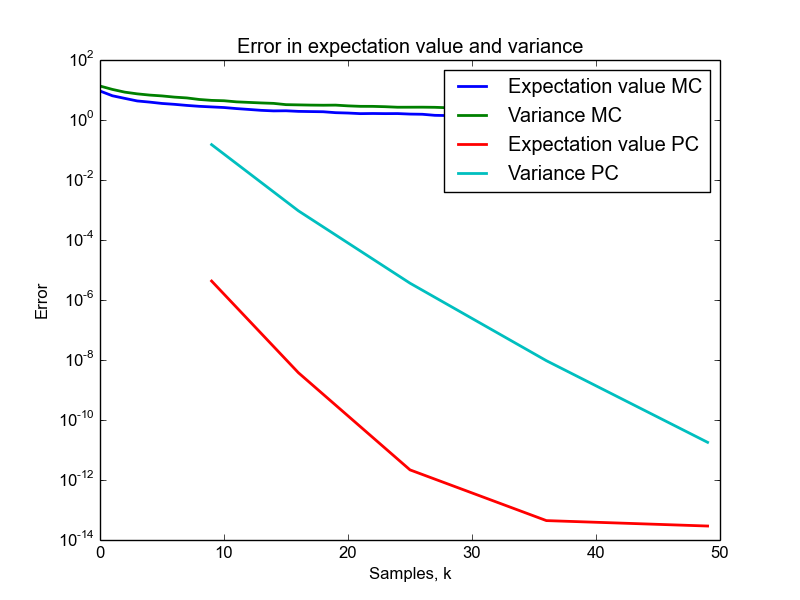
\includegraphics[width=0.7\textwidth]{MC_convergence_2D.png}
 \end{figure}

\end{frame}



\begin{frame}
 \frametitle{Introducing the pseudo-spectral approach}
 % TODO
 % med: subscript all f and F with Q, e.g. f_Q and F_Q

 \begin{align*}
     c_n(x) &= \frac{\inner{ u,P_n}}{\norm{P_n}^2}\\
\onslide<2-> {&=\frac{1}{\norm{P_n}^2} \int u(x,q)P_n(q)f_Q(q)dq} \onslide<3-> {\approx\\
\hat{c}_n(x) &= \frac{1}{\norm{P_n}^2} \sum_{k=0}^K
P_n(q_k)u(x,q_k)f(q_k)\omega_k}
\end{align*}\pause\pause
\begin{itemize}
    \item[$q_k$] quadrature nodes
\item[$\omega_k$] quadrature weights
\end{itemize}

 \end{frame}


     
\begin{chaospy}{Generating nodes and weights in Chaospy}
     % TODO
     % high: add code for 1-D gen_quad
     % high: list quadrature schemes
    \scriptsize
\onslide<1->
\begin{lstlisting}[language=python]
dist = cp.Normal()
nodes, weights = cp.generate_quadrature(2, dist, rule="G")
print nodes
[[-1.73205081  0.          1.73205081]]
print weights
[ 0.16666667  0.66666667  0.16666667]
\end{lstlisting}
\normalsize
\onslide<2->
 
\begin{table}
\caption{Quadrature rules:} 
\begin{tabular}{|ll|l|}
\hline
 Key & & Description\\\hline
    "Gaussian"& "G" &    Optimal Gaussian quadrature.\\
    "Legendre"& "E" &    Gauss-Legendre quadrature\\
    "Clenshaw"& "C" &    Clenshaw-Curtis quadrature.\\
    "Leja"& ``J" &          Leja quadrature.\\
    "Genz"& "Z" &        Hermite Genz-Keizter 16 rule.\\
    "Patterson" & "P"&    Gauss-Patterson quadrature rule.\\\hline
\end{tabular}
\end{table}

\end{chaospy}
 
 \begin{chaospy}{Generating nodes and weights in Chaospy}
     % TODO
     % high: add code for 1-D gen_quad
     % high: list quadrature schemes
    \scriptsize
\begin{lstlisting}[language=python]
dist = cp.Uniform()
nodes, weights = cp.generate_quadrature(2, dist, rule="G")
print nodes
[[ 0.11270167  0.5         0.88729833]]
print weights
[ 0.27777778  0.44444444  0.27777778]
\end{lstlisting}
\normalsize
 
\begin{table}
\caption{Quadrature rules:} 
\begin{tabular}{|ll|l|}
\hline
 Key & & Description\\\hline
    "Gaussian"& "G" &    Optimal Gaussian quadrature.\\
    "Legendre"& "E" &    Gauss-Legendre quadrature\\
    "Clenshaw"& "C" &    Clenshaw-Curtis quadrature.\\
    "Leja"& ``J" &          Leja quadrature.\\
    "Genz"& "Z" &        Hermite Genz-Keizter 16 rule.\\
    "Patterson" & "P"&    Gauss-Patterson quadrature rule.\\\hline
\end{tabular}
\end{table}

\end{chaospy}
 
%  \begin{chaospy}{Repetition: 2D code}
%  
%   \begin{lstlisting}[language=python]
%  def u(x,a, I):
%    return I*np.exp(-a*x)
%  |\pause| 
%  a = cp.Uniform(0, 0.1); I = cp.Uniform(8, 10)
%  dist = cp.J(a,I)|\pause|
%  x = np.linspace(0, 10, 100)
%  m = 2
%  |\pause| 
%  P = cp.orth_ttr(m, dist)|\pause|
%  nodes, weights = cp.generate_quadrature(m+1, dist,
%                                          rule="G")|\pause|
%  i1,i2 = np.mgrid[:len(weights), :100]|\pause|
%  solves = u(x[i2],nodes[0][i1],nodes[1][i1])|\pause|
%  u_hat = cp.fit_quadrature(P, nodes, weights,
%                            solves)
%  \end{lstlisting}
%  \end{chaospy}

\begin{frame}
 \frametitle{Quadrature rule $\Pi$}
 \begin{table}
  \begin{tabular}{lcccccccc}
    $\Pi_0$& &&& $\bullet$& &&&  \\\hline
   $\Pi_1$ &&&$\bullet$& &$\bullet$&&& \\\hline
   $\Pi_2$ &&$\bullet$&&$\bullet$ &&$\bullet$&& \\
   \end{tabular}
\end{table}  \pause
  
\begin{alert}
    {Multivariate combinations:}
  \[\Pi_{11} = \begin{array}{cccc}
                 \bullet & & \bullet\\
                 &&\\
                 \bullet & & \bullet
                 \end{array}
\]
 \[ \Pi_{20} = \begin{array}{ccccc}
           \bullet & & \bullet & & \bullet
          \end{array} \qquad \Pi_{12} = \begin{array}{cccc}
					\bullet&&\bullet\\
					\bullet&&\bullet\\
					\bullet&&\bullet\\
                                        \end{array}
 \]
\end{alert}
\pause
\begin{itemize}
    \item[$K$] Total number of quadrature nodes
    \item[$L$] Quadrature order along an axis
\end{itemize}
 \end{frame}

 \begin{chaospy}{Generating multivariate integration rules in
     Chaospy}
     \scriptsize
 % TODO
% high: fill in code (using L as input)
% skip "rule="
\begin{lstlisting}[language=python]
dist = cp.J(cp.Uniform(),cp.Uniform())
nodes, weights = cp.generate_quadrature((1,2), dist, rule="G")

print nodes
[[ 0.21132487  0.21132487  0.21132487  0.78867513  0.78867513  0.78867513]
 [ 0.11270167  0.5         0.88729833  0.11270167  0.5         0.88729833]]
 
print weights
 [ 0.13888889  0.22222222  0.13888889  0.13888889  0.22222222  0.13888889]
\end{lstlisting}

\end{chaospy}


%  \begin{frame}
%   \frametitle{Plot of the nodes for the 2D problem, $\Pi_{44}$}
%   \begin{figure}
%    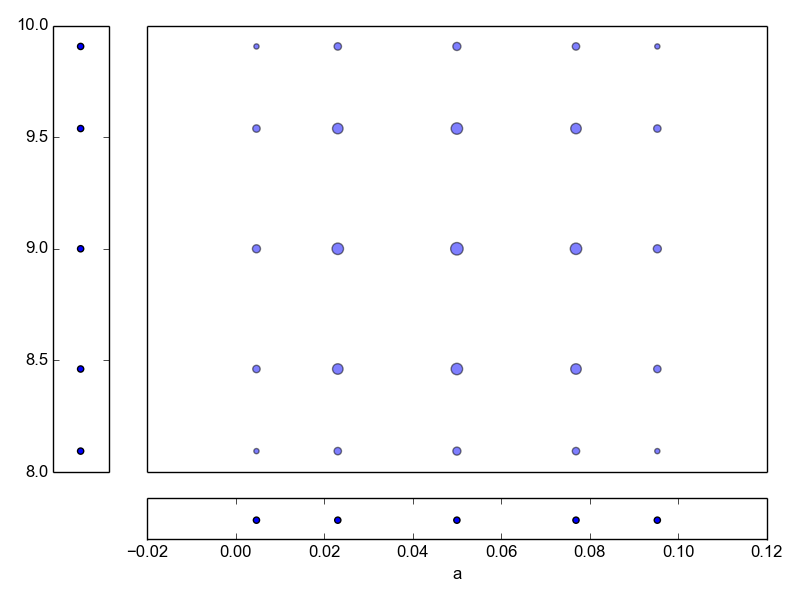
\includegraphics[width=0.85\textwidth]{nodes.png}
%   \end{figure}
%  \end{frame}


\begin{frame}
 \frametitle{Tensor products are sensitive to the curse of dimensionality}
 % TODO
 % high: Axes label: "quadrature order, L" vs "Total order, K"
 \begin{figure}
  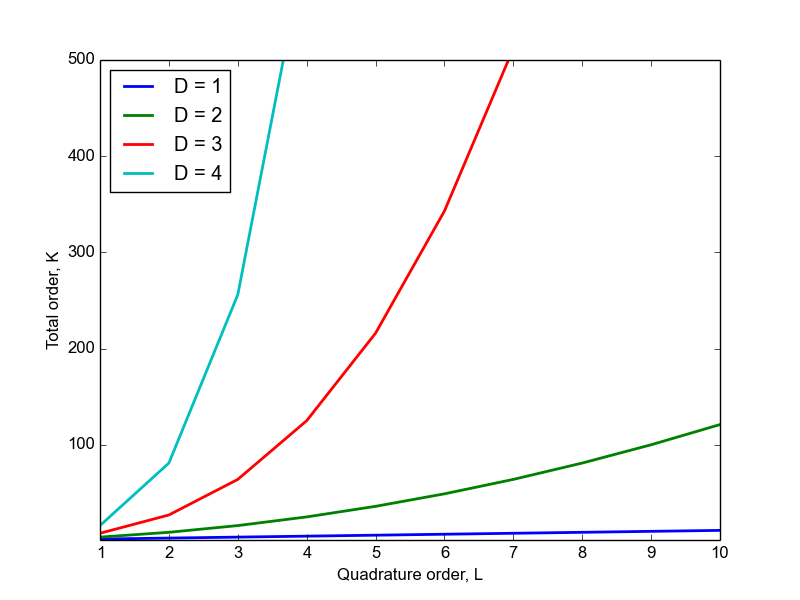
\includegraphics[width=0.85\textwidth]{dimensionality_nodes.png}
 \end{figure}
\end{frame}

\begin{frame}
 \frametitle{Smolyak sparse grids can drastically reduce the
 number of samples}
 \pause
Full tensor basis:
\begin{table}
 \begin{tabular}{|c|c|c|}\hline
 $y^2$&$y^2x$&$y^2x^2$\\\hline
 $y$&$yx$&$yx^2$\\\hline
 $1$&$x$&$x^2$\\\hline
 \end{tabular}
\end{table}
\pause
Smolyak sparse grid:
 \begin{figure}
  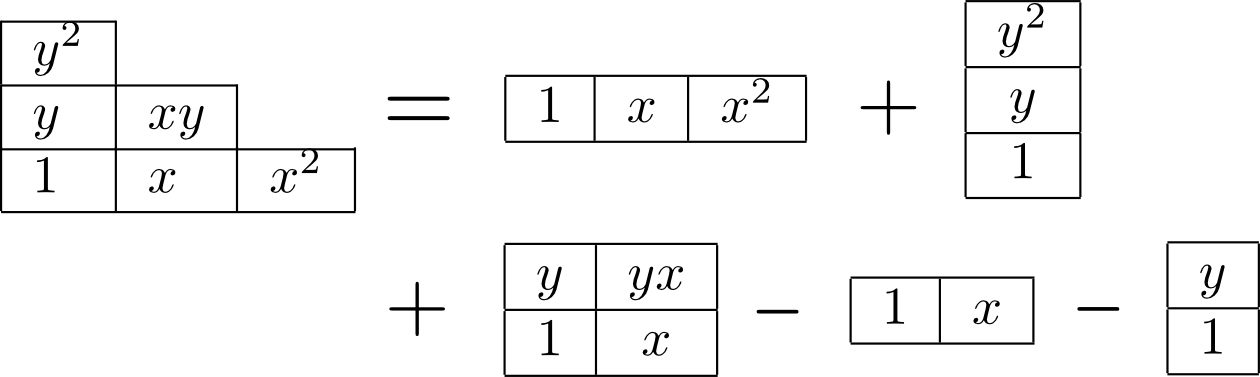
\includegraphics[width=0.9\textwidth]{smolyak2.png}
 \end{figure}
\[\Pi_{20} + \Pi_{11} + \Pi_{02} - \Pi_{10} - \Pi_{01}\]
\end{frame}


\begin{frame}
 \frametitle{Example of a Smolyak node placement}
    % TODO ???
    % high: røde prikkene er plassert feil
 \begin{figure}
  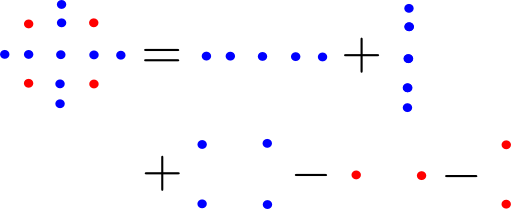
\includegraphics[width=\textwidth]{smolyak.png}
 \end{figure}

\end{frame}


\begin{frame}[fragile]
 \frametitle{Creating sparsegrid nodes in Chaospy}
 \begin{lstlisting}[language=python]
  nodes, weights = 
   cp.generate_quadrature(k, dist, rule="G",
                          sparse=True)
 \end{lstlisting}

 \pause
 \begin{figure}
  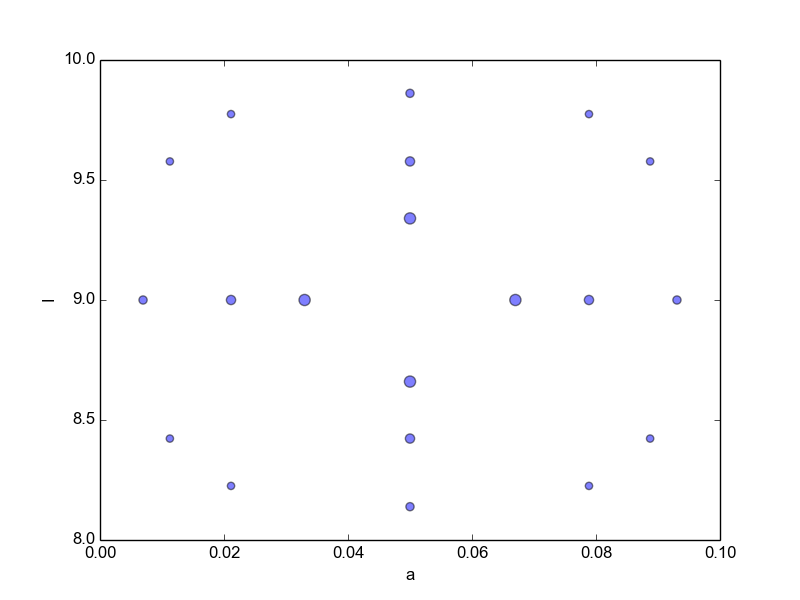
\includegraphics[width=0.6\textwidth]{nodes_sparse.png}
 \end{figure}
\end{frame}

\begin{frame}{Comparison between number of nodes using full tensor grid and sparse grid}{}
    % TODO
    % high: L vs K between GQ full tensor and GQ sparse grid
     \begin{figure}
  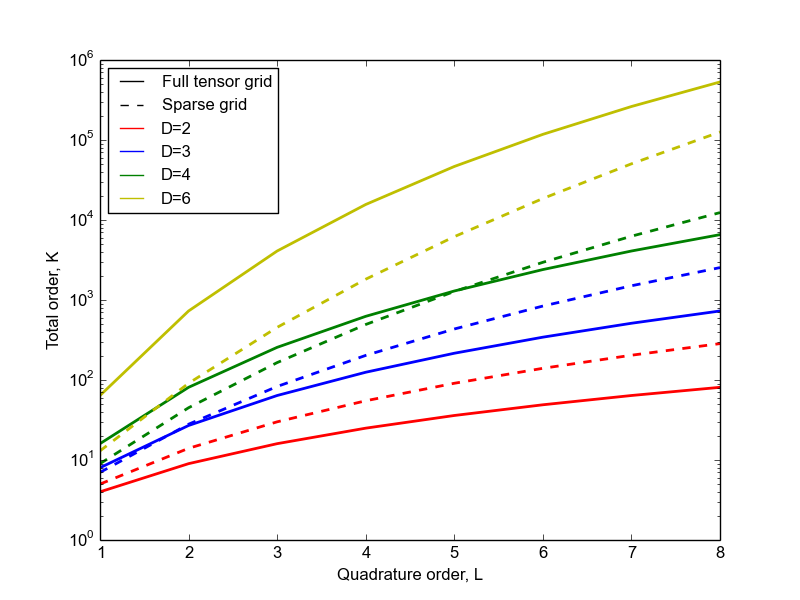
\includegraphics[width=0.85\textwidth]{dimensionality_nodes_gq_sparse.png}
 \end{figure}
\end{frame}
 
%  \begin{frame} 
%    \begin{figure}
%    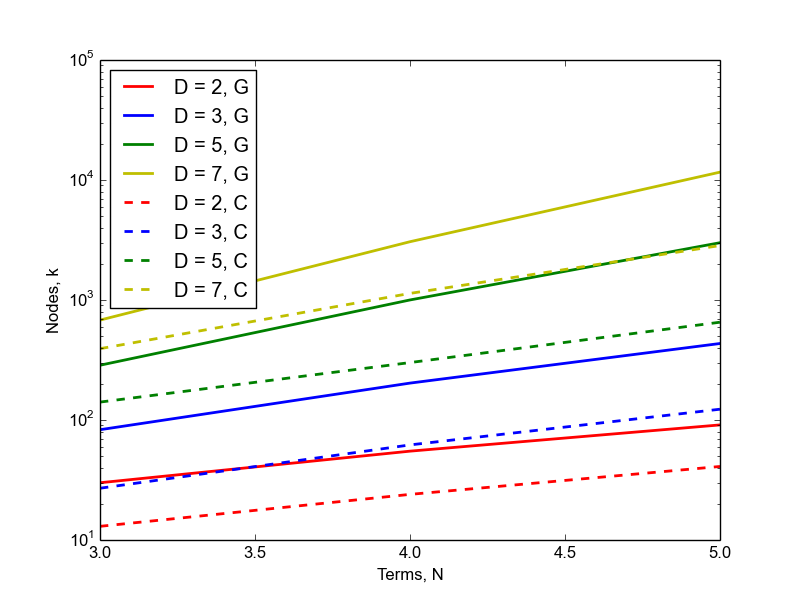
\includegraphics[width=0.85\textwidth]{dimensionality_nodes_sparse.png}
%   \end{figure}
%   \end{frame}
 
 \begin{frame}
  \frametitle{Nested sparse grids uses overlapping nodes to reduce
  the number of nodes further}
  
  \begin{alert}
      {Clenshaw-Curtis:}\\
      \scriptsize
     \verb;cp.generate\_quadrature(l, dist, rule="C", growth=False);
    \normalsize
  \begin{table}
  \begin{tabular}{lcccccccc}
    $\Pi_0$& &&& $\bullet$& &&&  \\\hline
   $\Pi_1$ &&&$\bullet$& &$\bullet$&&& \\\hline
   $\Pi_2$ &&$\bullet$&&$\bullet$ &&$\bullet$&& \\
   \end{tabular}
  \end{table}
  \end{alert}
  \pause
  \begin{alert}
      {Nested Clenshaw-Curtis:}\\
      \scriptsize
    \verb;cp.generate\_quadrature(l, dist, rule="C", growth=True);
    \normalsize
  \begin{table}
  \begin{tabular}{lcccccccc}
    $\Pi_0$& &&& $\bullet$& &&&  \\\hline
   $\Pi_1$ &&$\bullet$&& $\bullet$&&$\bullet$ && \\\hline
   $\Pi_2$ &$\bullet$&$\bullet$&$\bullet$& $\bullet$&$\bullet$&$\bullet$ &$\bullet$& \\
   \end{tabular}
  \end{table}
  \end{alert}
 
  \end{frame}

\begin{frame}
 \frametitle{Nested smolyak sparse grid in practice}


 \begin{figure}
  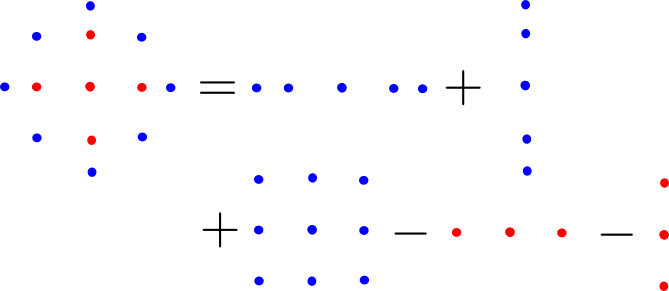
\includegraphics[width=\textwidth]{smolyak_nested.png}
 \end{figure}

\end{frame}

\begin{frame}
 \frametitle{The number of overlapping nodes grows quickly}
 \begin{figure}
  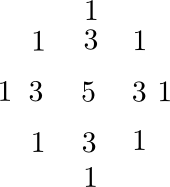
\includegraphics[width=0.5\textwidth]{smolyak_nested_nr.png}
 \end{figure}

\end{frame}

%   \begin{frame}
%   \frametitle{Clenshaw-Curtis quadrature vs Gaussian quadrature}
%   % TODO ???
%   % med: smaller figsize
%   % med: order (3,3)
%   \begin{columns}
%       \column{.5\textwidth}
%  \begin{center}
%                  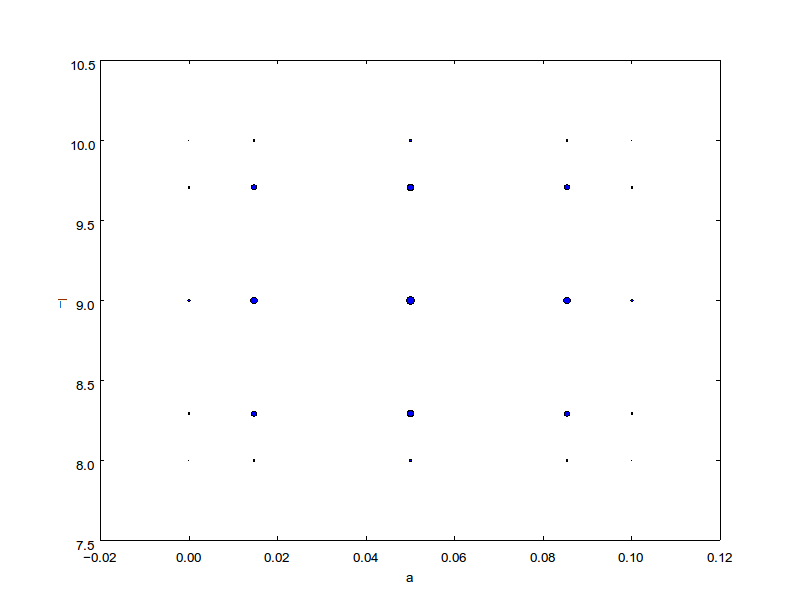
\includegraphics[width=\textwidth]{nodes_C.png}
%  
%                  {Clenshaw-Curtis quadrature}
%  \end{center}
%       \column{.5\textwidth}
%       \begin{center}
%                  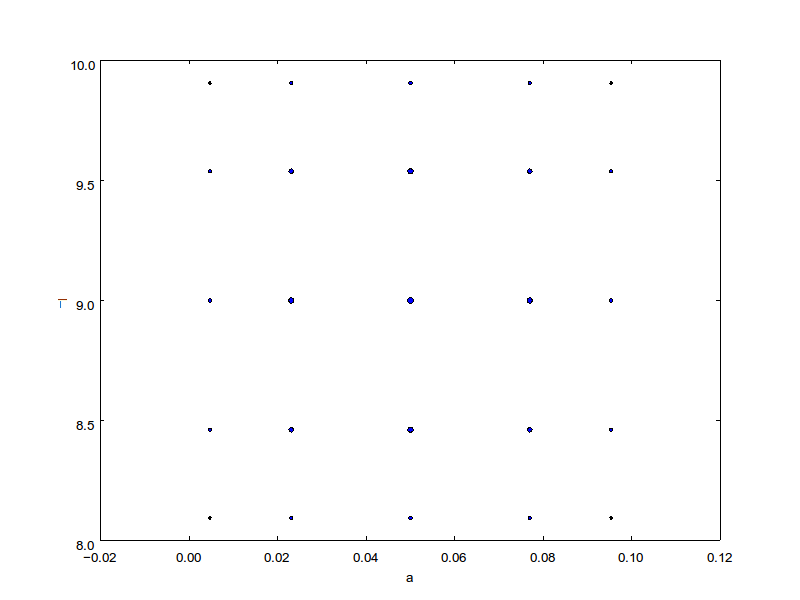
\includegraphics[width=\textwidth]{nodes_G.png}
%  
%                  {Gaussian quadrature}
%       \end{center}
%   \end{columns}
%  \end{frame}
 
 \begin{frame}
  \frametitle{Comparing the three methods}

 \begin{figure}
  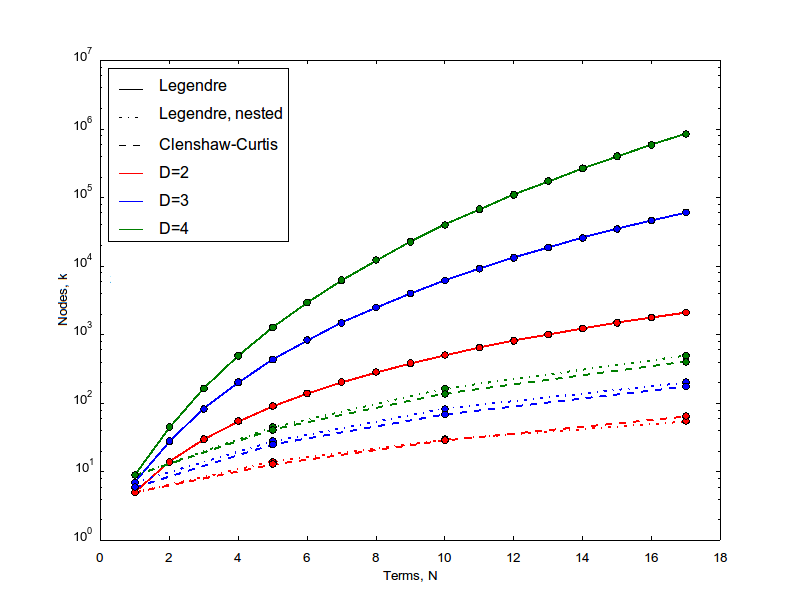
\includegraphics[width=0.85\textwidth]{dimensionality_nodes_nested.png}
 \end{figure}
 \end{frame}

  
  \begin{frame}
   \frametitle{Mapping between polynomial order $M$ and quadrature order $L$}
   For nested Clenshaw-Curtis
   \begin{figure}
    \includegraphics<1>[width=0.85\textwidth]{LvsM1.png}
    \includegraphics<2>[width=0.85\textwidth]{LvsM.png}
   \end{figure}

   
  %\begin{tabular}{lccccccccccc}
  % Order, M & 0 & 1 & 2 & 3 & 4 & 5 & 6 & 7 & 8 \\\\
  % Quad  & 1 & 4 & 9 & 16 & 25 & 36 & 49 & 64 & 81 \\\\
  % Poly  & 1 & 3 & 6 & 10 & 15 & 21 & 28 & 37 & 37
  %\end{tabular}

  \end{frame}

  
  
  \begin{frame}
 \frametitle{Difference between sparse grid and non nested sparse grid}
 \begin{center}
                 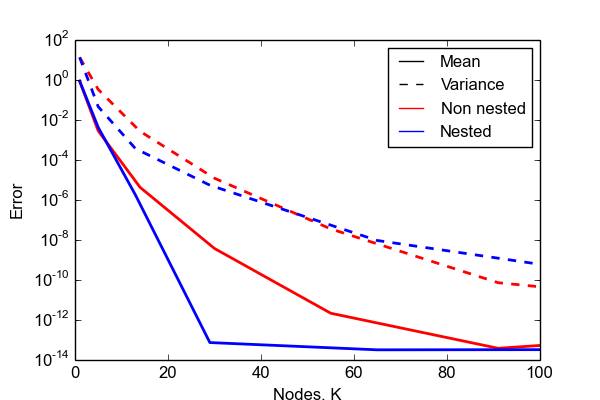
\includegraphics[width=0.85\textwidth]{convergence_2D_L_sparse.png}

 %                 $L=M-2$, $L=M-1$, $L=M$}
          \end{center}
 % TODO ???
 % effect not capture for sparse. Need M-2 at least
 % in full tensor: >>> plt.ylim(10**-14, 10**2)
%      \begin{columns}
%          \column{.5\textwidth}
%          \begin{center}
%                 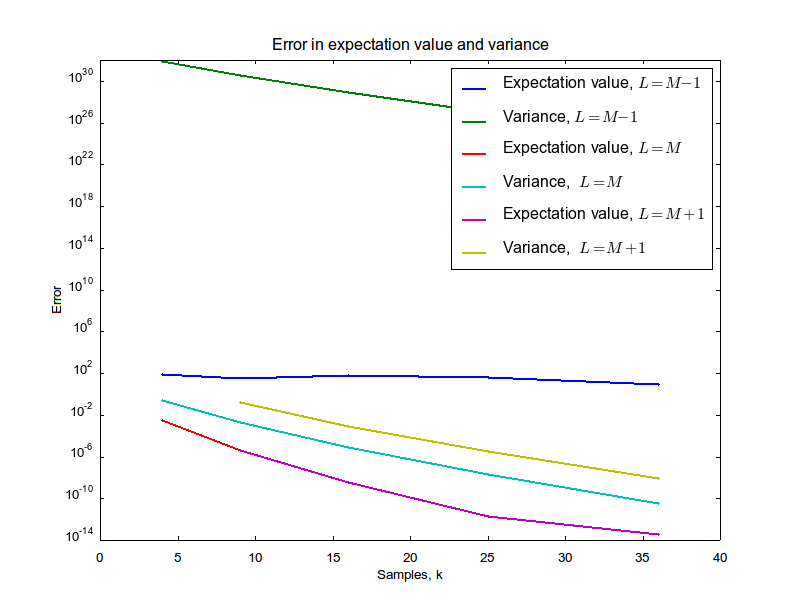
\includegraphics[width=\textwidth]{convergence_2D_L.png}
% 
%                 {Full tensor grid:}
% %                 $L=M-1$, $L=M$, $L=M+1$}
%          \end{center}
%          \column{.5\textwidth}
% 
%          \begin{center}
%                 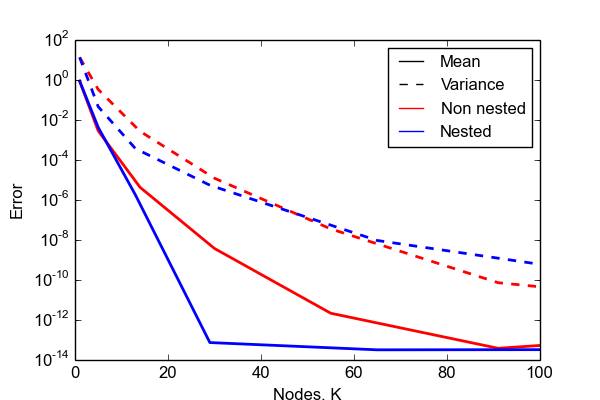
\includegraphics[width=\textwidth]{convergence_2D_L_sparse.png}
% 
%                 {Sparse grid:}
% %                 $L=M-2$, $L=M-1$, $L=M$}
%          \end{center}
%      \end{columns}
\end{frame}
  
  
  
 \begin{frame}
  \frametitle{Definition of Gaussian quadrature}
  \begin{align*}
   \int W(q)u(x,q)dq &\approx \sum_k \omega_k u(x,q_k)\\
   \intertext{for a weighting function $W(q)$}
   \uncover<2-> {\int f(q)u(x,q)dq \approx \sum_k \omega_k u(x,q_k)}
    \end{align*}
   \end{frame}

 
  \begin{frame}
 \frametitle{Nodes for different probability distributions}
 \begin{columns}
     \column{.5\textwidth}
     \begin{center}
                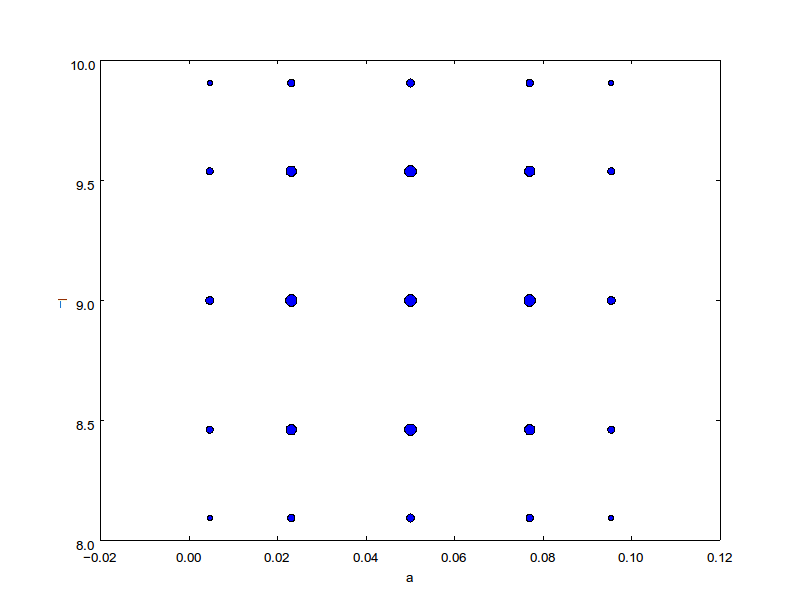
\includegraphics[width=.7\textwidth]{nodes_uniform.png}

                Uniform
     \end{center}

     \begin{center}
                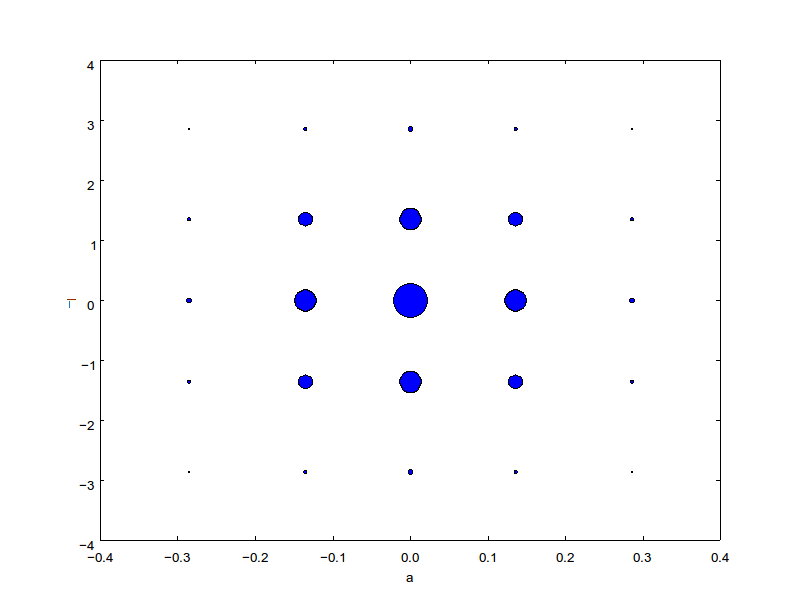
\includegraphics[width=.7\textwidth]{nodes_normal.png}

                Normal
     \end{center}
     \column{.5\textwidth}
     \begin{center}
                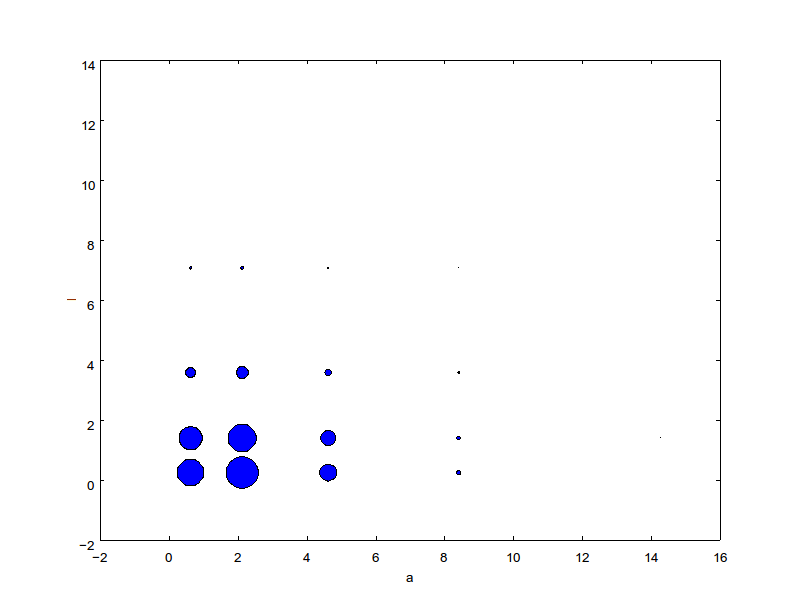
\includegraphics[width=.7\textwidth]{nodes_gamma.png}

                Gamma
     \end{center}

     \begin{center}
                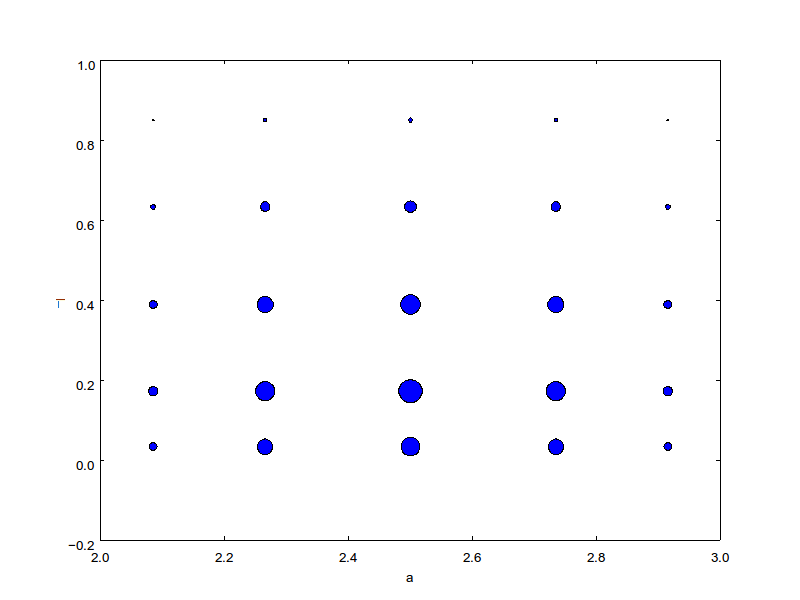
\includegraphics[width=.7\textwidth]{nodes_beta.png}

                Beta
     \end{center}
 \end{columns}
\end{frame}
 
 
%  \begin{frame}
%   \frametitle{Convergence for Gaussian quadrature vs Legendre}
%   % TODO ???
%   % What Gaussian? What problem?
%   \begin{figure}
%    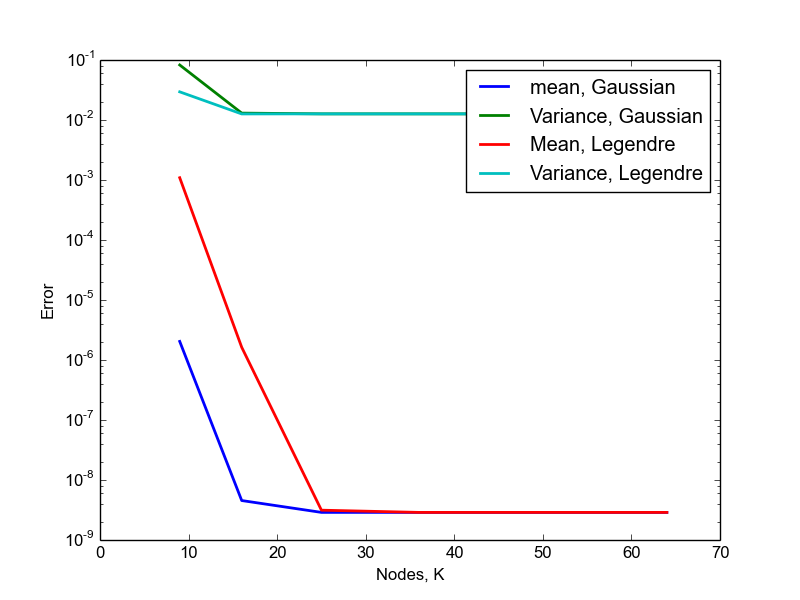
\includegraphics[width=0.85\textwidth]{convergence_GvsL.png}
%   \end{figure}
% 
%  \end{frame}

 
 \begin{frame}
  \frametitle{Point collocation method, the alternative to
  pseudo-spectral method}
  \pause
  \begin{align*}
      \bm c &= 
      \begin{bmatrix}
          c_0(x)\\\vdots\\c_N(x)
      \end{bmatrix}
      &
      \bm P &=
      \begin{bmatrix}{}
          P_0(q_0) & \cdots & P_N(q_0) \\
          \vdots & & \vdots \\
          P_0(q_K) & \cdots & P_N(q_K) \\
      \end{bmatrix}
      &
      \bm u &=
      \begin{bmatrix}{}
          u(x; q_0) \\ \vdots \\ u(x, q_K)
      \end{bmatrix}
  \end{align*}
  \pause
  \begin{align*}
      \bm{\hat c} &= \argmin_{\bm c} \|\bm P\bm c -\bm u\|_2^2 \\
      \onslide<4>{&= (\bm P^T\bm P)^{-1} \bm P^T \bm u}
  \end{align*}
 
 \end{frame}

\begin{frame}
 \frametitle{Collocation nodes should be placed where probability is high}
 \begin{figure}
  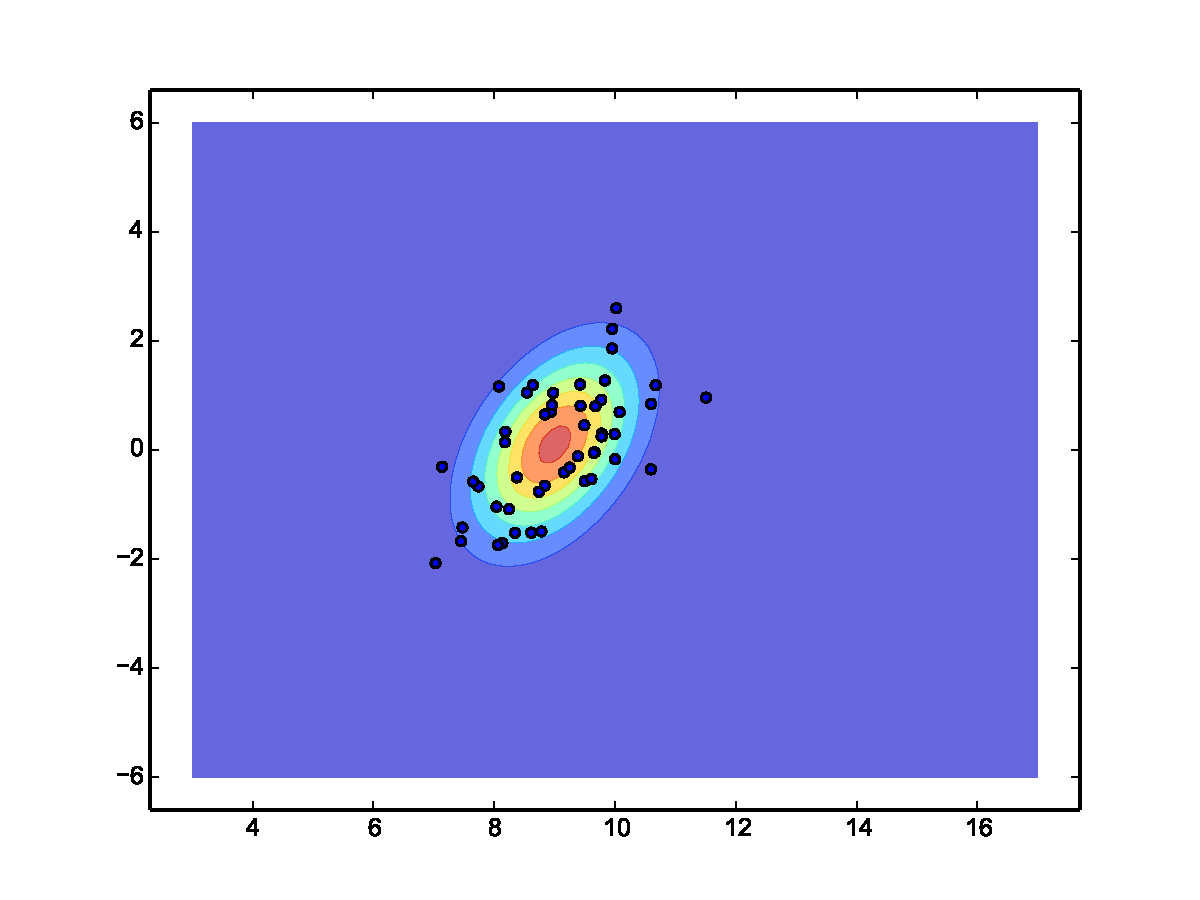
\includegraphics[width=0.85\textwidth]{sampling.pdf}
 \end{figure}
 
\end{frame}

\begin{chaospy}{Code for least square minimization}
    % TODO 
    % remove "H" and rule="LS" and simulate again again.
    \scriptsize
 \begin{lstlisting}[language=python]
def u(x, a, I):
  return I*np.exp(-a*x)
 |\pause|
a = cp.Uniform(0, 0.1)
I = cp.Uniform(8, 10)
dist = cp.J(a,I)
|\pause|
M = 3
x = np.linspace(0, 10, 100)
 |\pause|
P = cp.orth_ttr(M, dist) |\pause|
nodes = dist.sample(2*len(P)) |\pause|
solves = [u(T, s[0], s[1]) for s in nodes.T] |\pause|
U_hat = cp.fit_regression(P, nodes, solves)
 \end{lstlisting}

\end{chaospy}

\begin{frame}
 \frametitle{Convergence using least square minimization}
 % TODO
 % Redo: only random samples (see prev. frame)
 \begin{figure}
  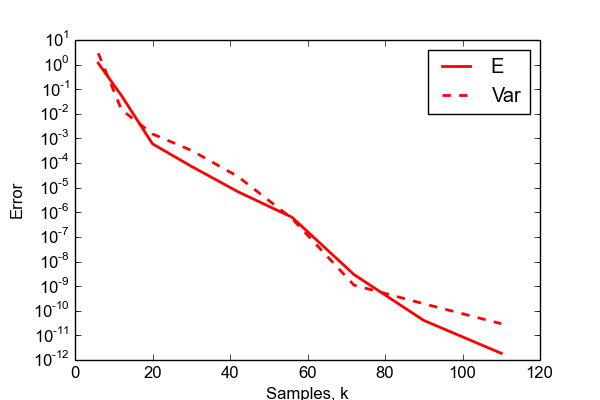
\includegraphics[width=0.85\textwidth]{convergence_collocation.png}
 \end{figure}
\end{frame}


  \begin{frame}[fragile]
 \frametitle{(Pseudo-)Random sampling schemes}
 % TODO
 % compare 4 schemes: ' ', 'M', 'S', 'L'
 % remove margins
 \begin{columns}
     \column{.5\textwidth}
     \begin{center}
                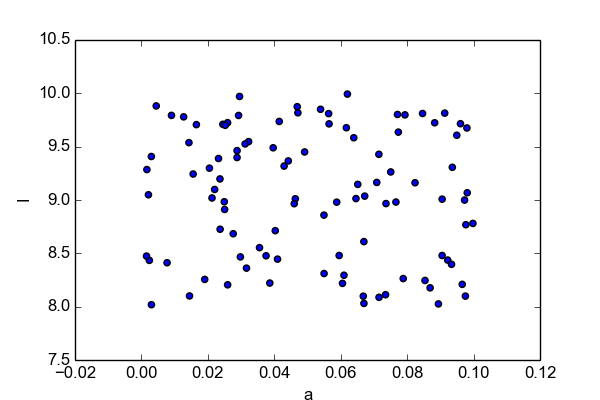
\includegraphics[width=0.7\textwidth]{samples.png}

                (Pseudo-)Random sampling, default:

                \scriptsize
                \verb;nodes = dist.sample(100);
                \normalsize
                %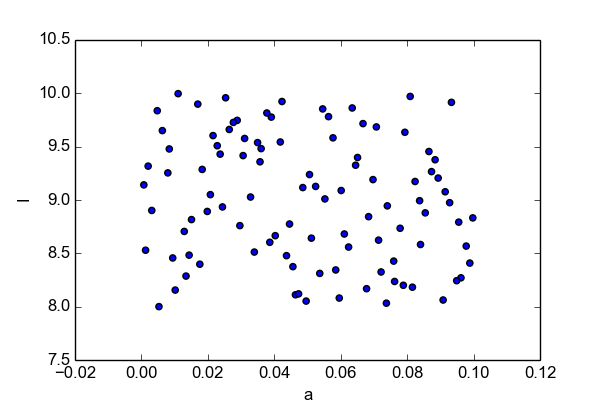
\includegraphics[width=0.7\textwidth]{samples_L.png}

                L sampling:

                \scriptsize
                \verb;nodes = dist.sample(100,"L");
                \normalsize
     \end{center}
     \column{.5\textwidth}
     \begin{center}
                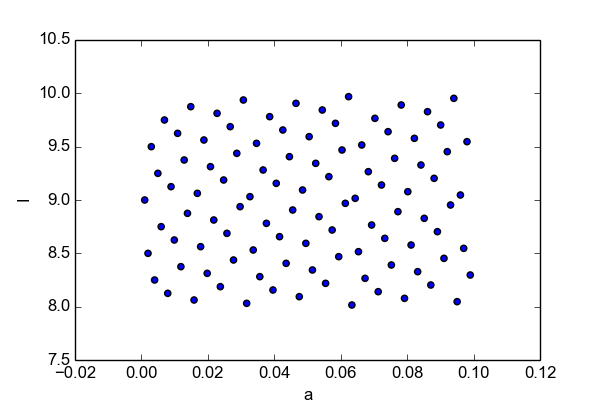
\includegraphics[width=0.7\textwidth]{samples_M.png}

                Hammersley sampling

                \scriptsize
                \verb;nodes = dist.sample(100, "H");
                \normalsize
                
                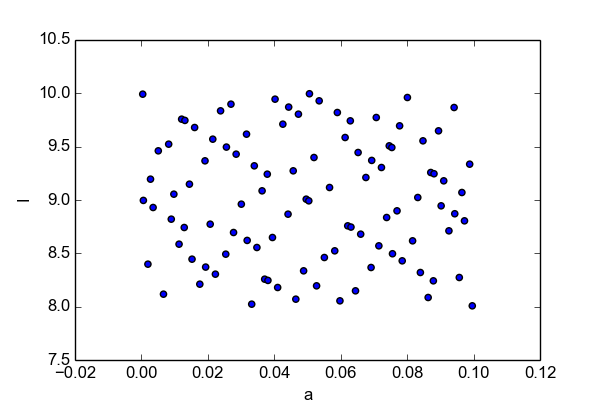
\includegraphics[width=0.7\textwidth]{samples_S.png}

                Sobol sampling

                \scriptsize
                \verb;nodes = dist.sample(100, "S");
                \normalsize
     \end{center}
 \end{columns}
\end{frame}


\begin{frame}
 \frametitle{Convergence using different sampling schemes}
 % TODO  ???
 % All 4 where ' ' and 'L' is done with bootstrapping
 % might want to subtract median reference
 % (Ask me about boostrapping)
  \begin{figure}
  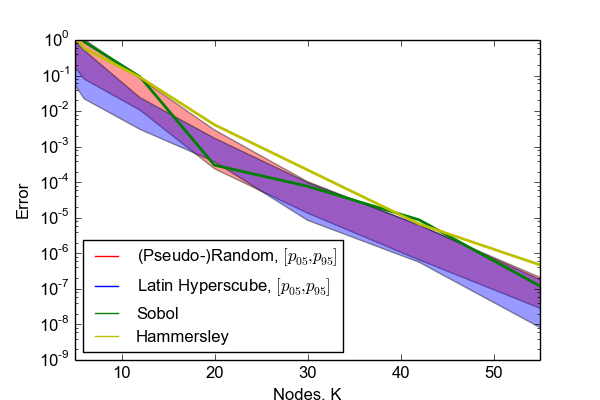
\includegraphics[width=0.85\textwidth]{convergence_collocation_compare.png}
 \end{figure}
\end{frame}

\begin{frame}{Too few samples can lead to inversion instabilities}
    % TODO
    % fix M and D
    % find K such that problem is unstable with LS and stable with T
    % 2 plots: LS and T separated with \pause
\end{frame}


\begin{frame}{A comparison between different methods}{}
    % TODO
    % Plot!
    % SC nested-CC sparsegrid vs. PC with S-rule and LS-fit vs. MC
      \begin{figure}
  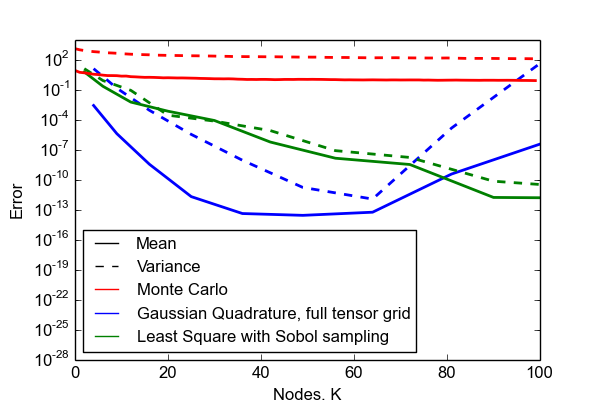
\includegraphics[width=0.85\textwidth]{MC_convergence_2D_diff.png}
 \end{figure}
\end{frame}

\begin{frame}{Which method to choose for your problem}{}
    \scriptsize
    \begin{tabular}{r|lll}
        & \bf Pseudo-spectral &
        \bf Point collocation & \bf Monte Carlo \\ \\ \hline \pause\\
        Efficiency              & \color{green} Highest
            & \color{green} Very high & \color{red} Very low  \pause\\\\
        Stability               & \color{red} Low
            & Medium   & \color{green}Very high \pause\\\\
            Dimension-independence  & \color{red} Lowest
            & \color{red} Low    & \color{green} Highest
    \end{tabular}
\end{frame}

\begin{chaospy}{A proxy model allows for computational cheap statistical analysis}
 \begin{lstlisting}[language=python]
mean =  cp.E(U_hat,dist)
var = cp.Var(U_hat,dist)
|\pause|

mean = c[0]
var = np.sum(norms[1:]*c[1:].T**2,1)
|\pause|

s = dist.sample(10**6)
u_mc = U_hat(*s)
mean = np.mean(u_mc,1)
var = np.var(u_mc,1)
\end{lstlisting}
\end{chaospy}

%  \begin{frame}
%   \frametitle{The three methods are almost identical}
%   % TODO
%   % Better legend (text and placement)
%   \begin{columns}
%       \column{.5\textwidth}
%     \begin{figure}
%      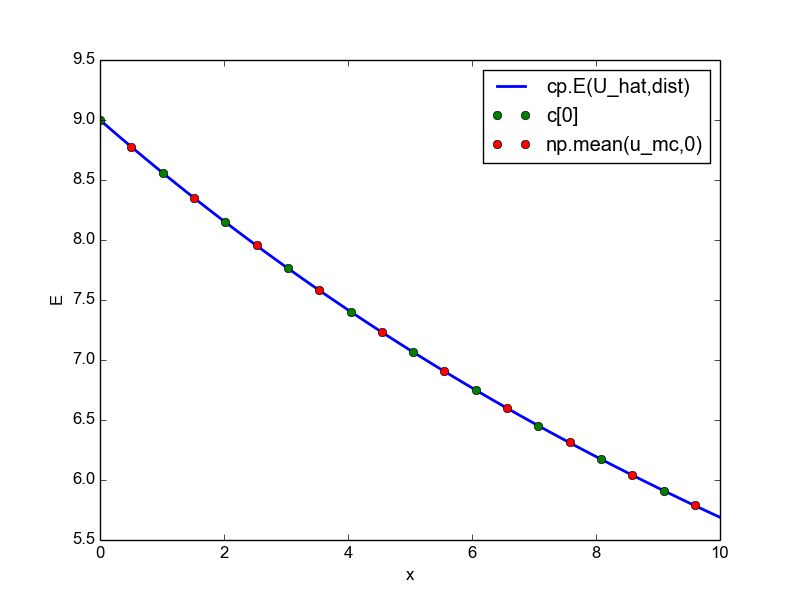
\includegraphics[width=\textwidth]{E.png}
%     \end{figure}
%       \column{.5\textwidth}
%     \begin{figure}
%      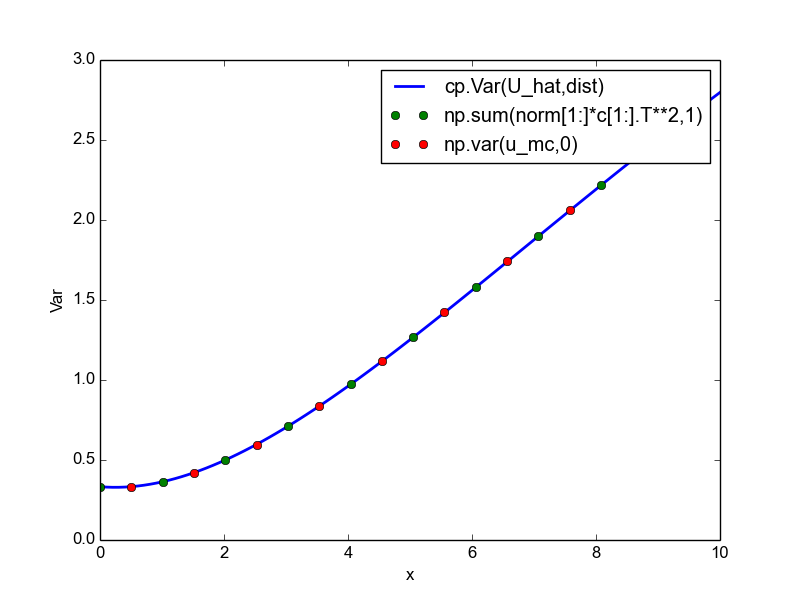
\includegraphics[width=\textwidth]{Var.png}
%     \end{figure}
%   \end{columns}
%  \end{frame}

\begin{frame}{Modelling bloodflow requires sensitivity analysis}{}
    \begin{columns}
        \column{.3\textwidth}
        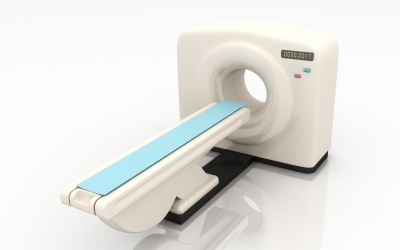
\includegraphics[width=\textwidth]{ntnu/ID-10015904.jpg}
        \column{.3\textwidth}
        
\includegraphics[width=\textwidth]{ntnu/STARFiSh-Logo_small_transparent.png}
        \column{.3\textwidth}
        
\includegraphics[width=\textwidth]{chaospy_logo.jpg}
    \end{columns} \pause
    \begin{center}
    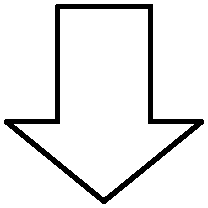
\includegraphics[width=.1\textwidth]{figures/south.pdf}
    \end{center}
    \begin{columns}
        \column{.5\textwidth}
        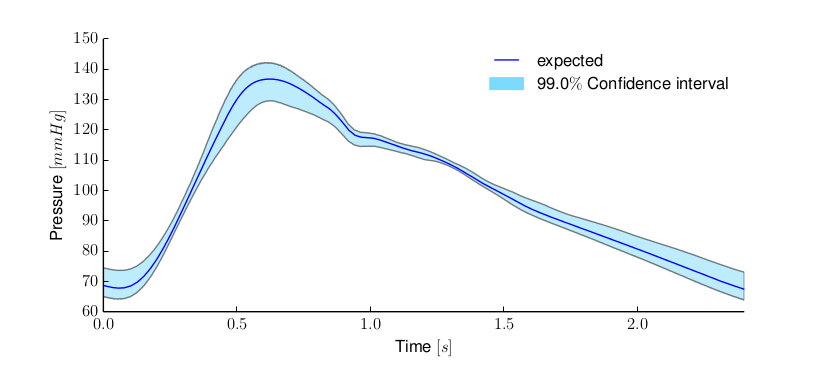
\includegraphics[width=\textwidth]{ntnu/AorticPressure_parameterUncertainty.png}
        \column{.5\textwidth}
        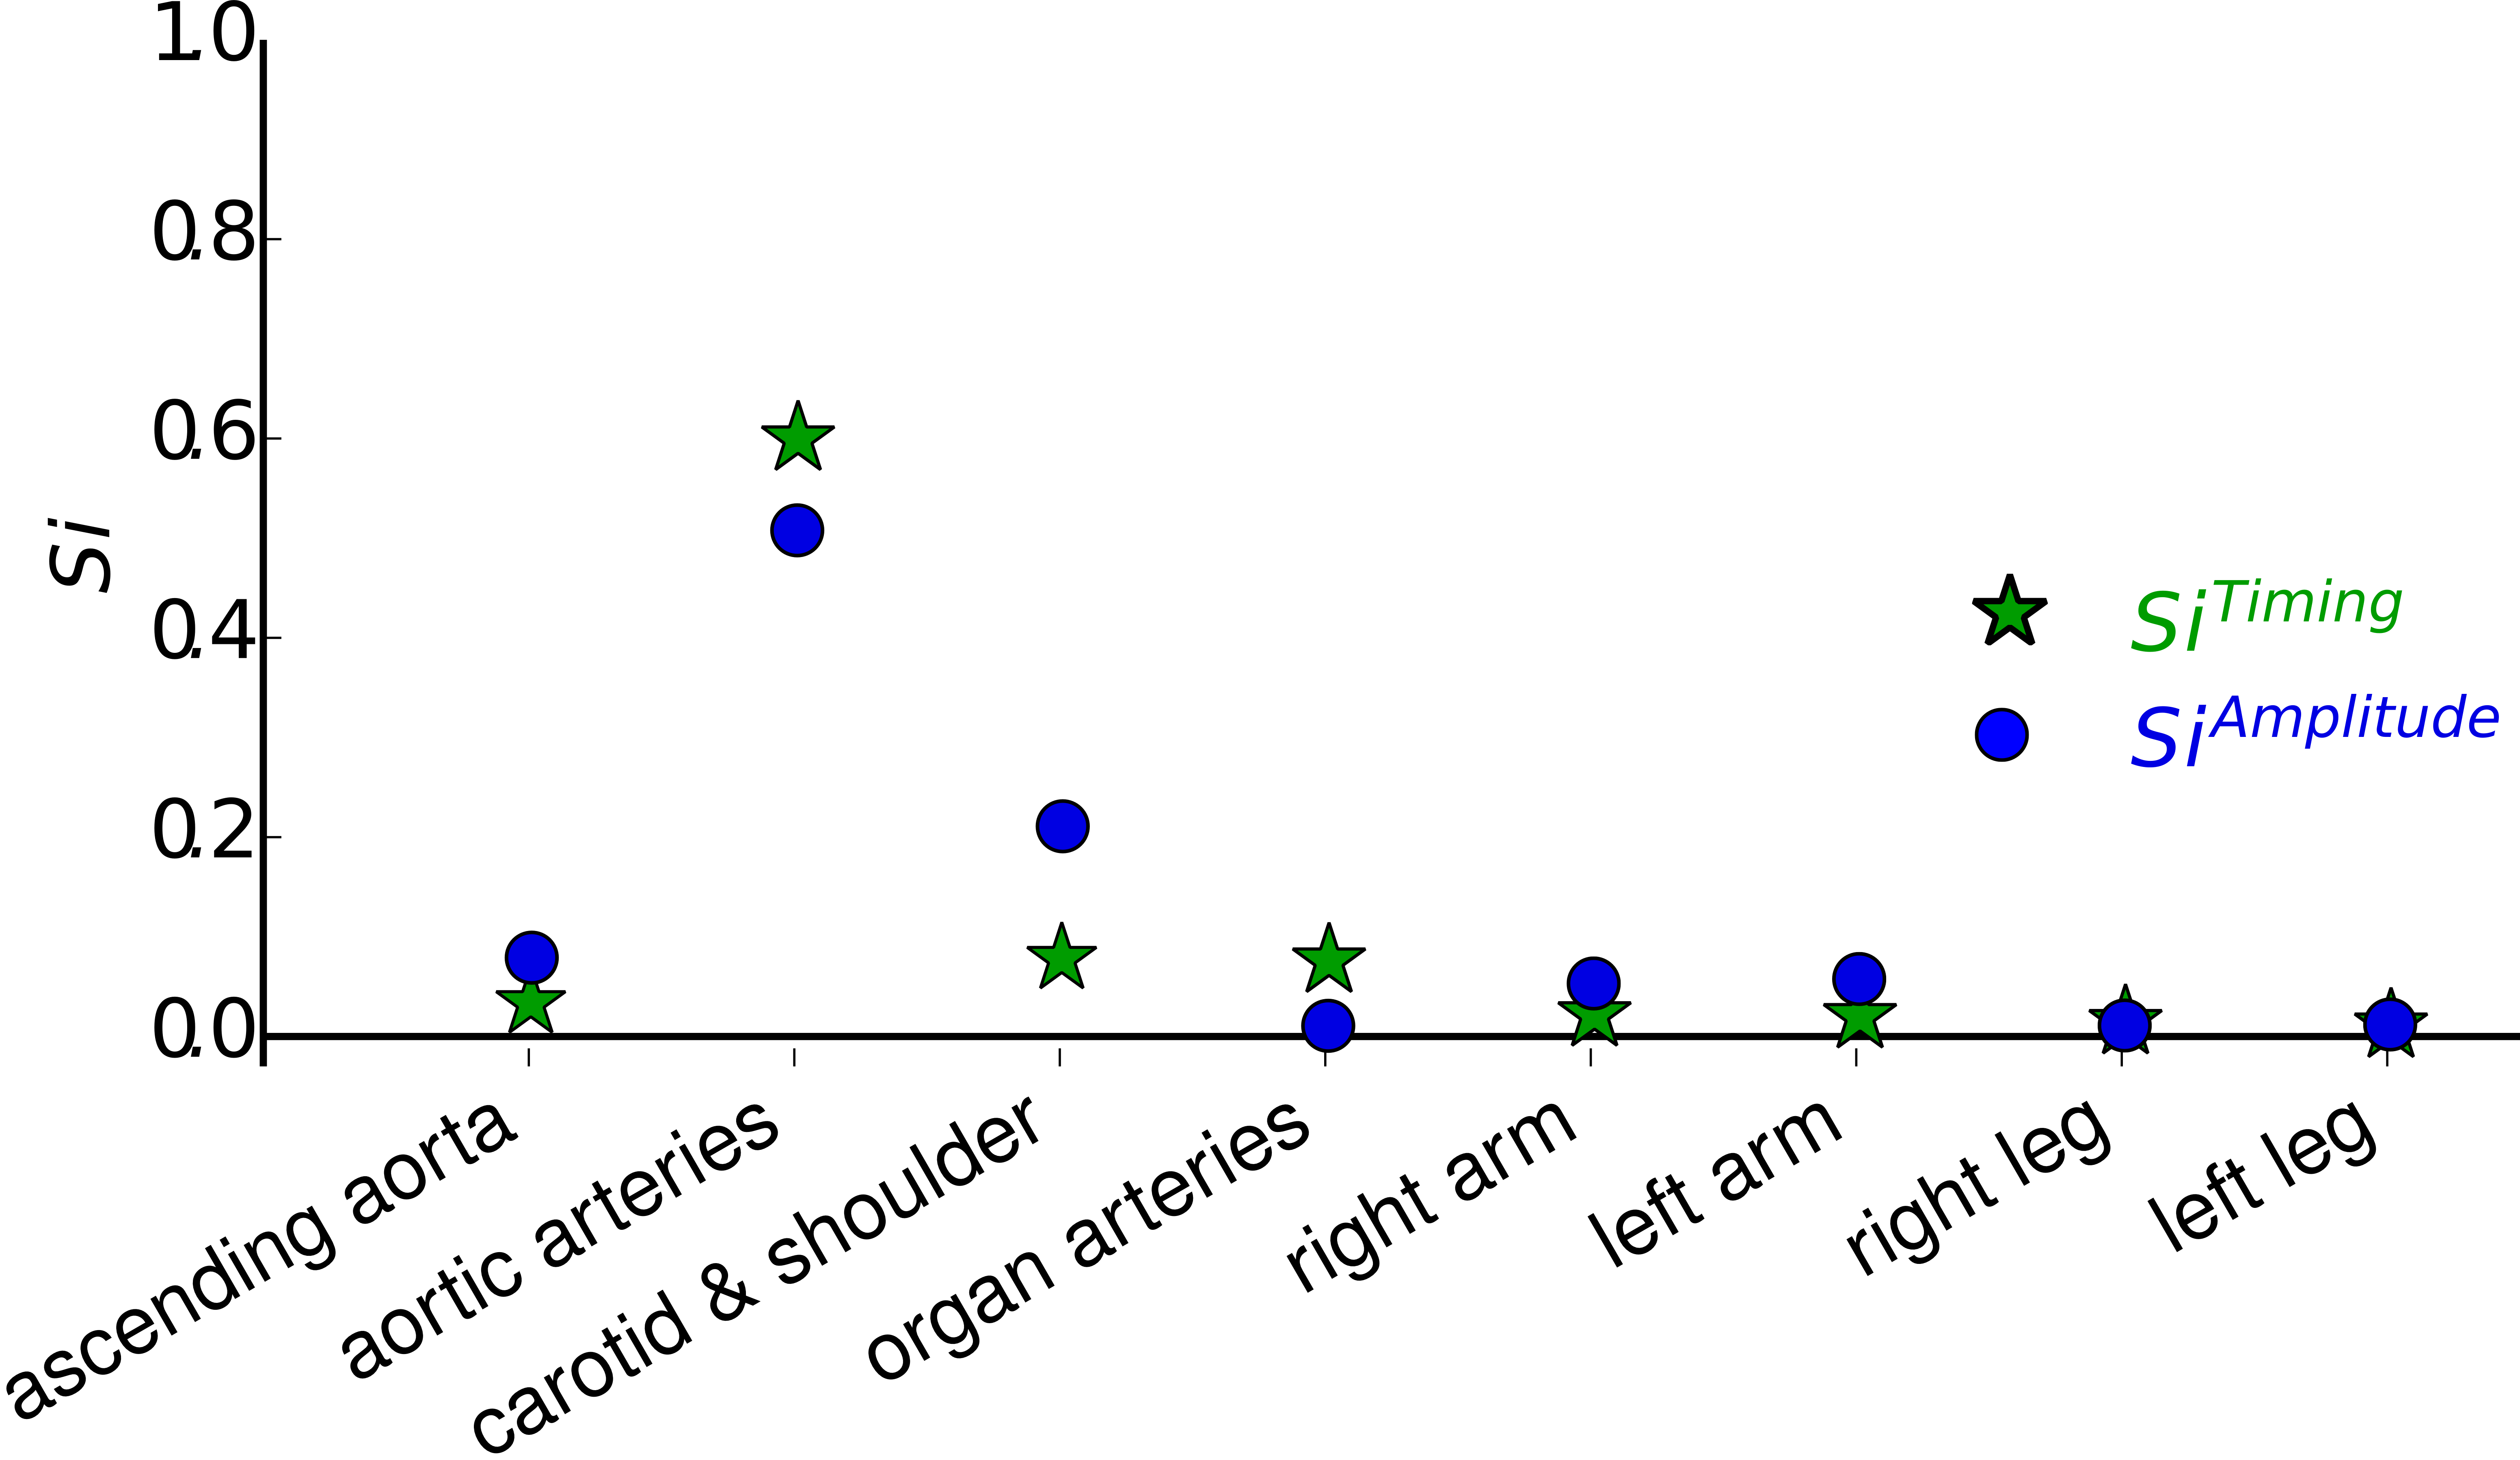
\includegraphics[width=\textwidth]{ntnu/results/sensitivity-pointOfinflection.png}
    \end{columns}
    \end{frame}

\begin{frame}[fragile]
 \frametitle{Polynomial chaos expansion designed for everything
 based on expected value $E$}
\begin{alert}
    {Variance based sensitivity:}
 \begin{align*}
  S_{T_i} &= \frac{\E{\Var{u | dist \backslash d_i }}}{\Var{u}}\\
\onslide<2->{&= \frac{\E{\E{u^2 | dist \backslash d_i } - \E{(u | dist \backslash d_i )^2}}}{\Var{u}}}
\end{align*} 
\end{alert}

\onslide<3->
\begin{alert}{Constructor:}

  \verb;S_Ti = cp.Sens_t(U_hat, dist);
\end{alert}

% \begin{alert}
%     {Manual code:} % TODO manual code D=2
% 
%   \verb;S_Ti = cp.Sens_t(U_hat, dist);
% \end{alert}
\end{frame}

\begin{chaospy}{Manual code for Variance based sensitivity}
\scriptsize
 \begin{lstlisting}[language=python]
D=2
zero = [1]*D
|\pause|
Sense = np.empty((D,) + U_hat.shape)|\pause|
V = cp.Var(U_hat, dist)|\pause|

for i in range(D):
    zero[i] = 0
    Sense[i] = (V-cp.Var(cp.E_cond(U_hat, zero, dist), dist))/V
    zero[i] = 1
 \end{lstlisting}

\end{chaospy}


\begin{frame}
 \frametitle{Variance based sensitivity of our naive example}
  \begin{figure}
  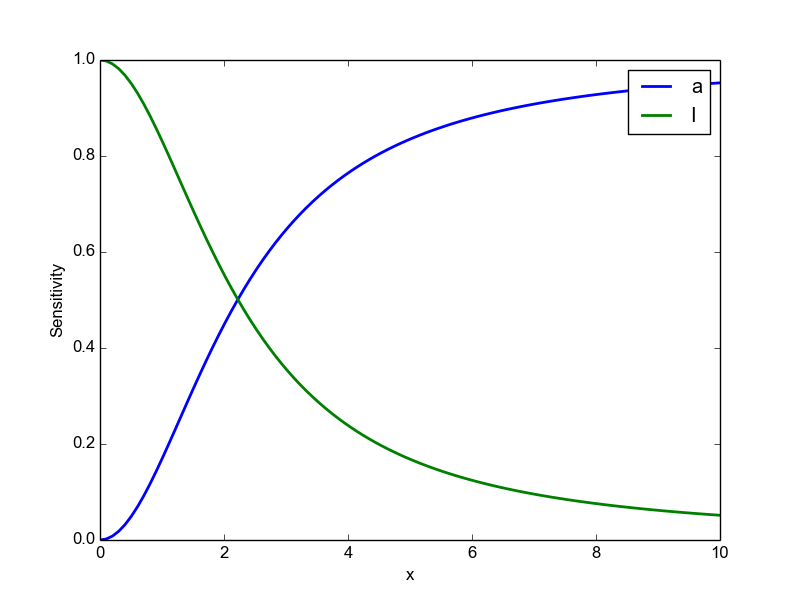
\includegraphics[width=0.85\textwidth]{sens.png}
 \end{figure}
\end{frame}

\begin{chaospy}{Polynomial chaos expansions for other metric is
    still possible}
    % TODO Manual code
    
\begin{lstlisting}[language=python]
u_mc =  np.sort(u_mc,1)
p_10 = u_mc[:,round(0.1*len(u_mc[0,:]))]
p_90 = u_mc[:,round(0.9*len(u_mc[0,:]))]
 \end{lstlisting}
 \pause
  \begin{lstlisting}[language=python]
p_10 = np.percentile(u_mc,10,1)
p_90 = np.percentile(u_mc,90,1)
 \end{lstlisting}
\end{chaospy}

\begin{frame}
 \frametitle{Confidence interval}
 % TODO
  \begin{figure}
  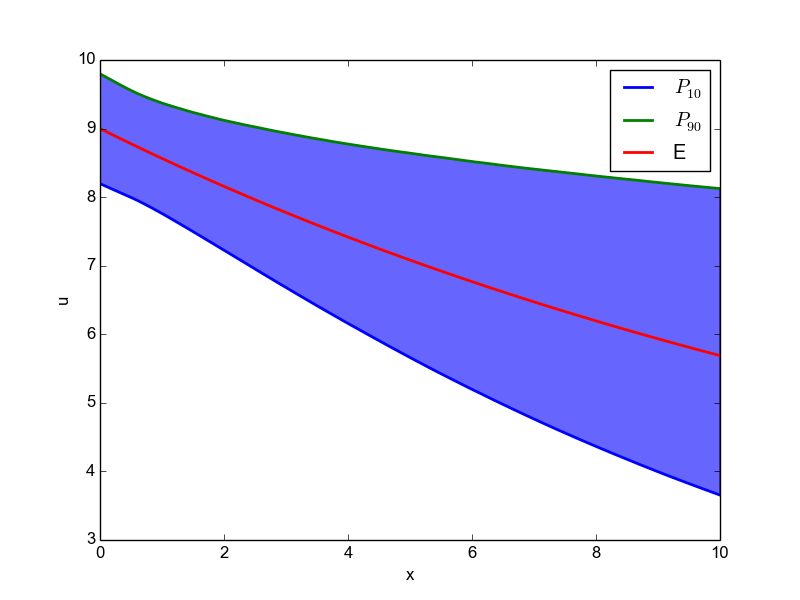
\includegraphics[width=0.85\textwidth]{percentiles.png}
 \end{figure}
 
\end{frame}


\begin{chaospy}{Summary}
    \scriptsize
 \begin{lstlisting}[language=python]
x = np.linspace(0, 10, 100)
def u(x, a, I):
  return I*np.exp(-a*x)
|\pause|
a = cp.Uniform(0, 0.1)
I = cp.Uniform(8, 10)
dist = cp.J(a,I)
|\pause|
P = cp.orth_ttr(M, dist)
|\pause|
nodes, weights = cp.generate_quadrature(M+1, dist)
|\pause|
solves = [u(x, s[0], s[1]) for s in nodes.T]
|\pause|
u_hat= cp.fit_quadrature(P, nodes, weights, solves)
|\pause|
mean = cp.E(u_hat, dist)
var = cp.Var(u_hat, dist)
\end{lstlisting}

\end{chaospy}


\end{document}
